\section {Routing}
\subsection {Routing}
\subsection {Routing}
\subsection {Routing}
\input{fig/pcb/routing}
We spent the entire final week before production working on the routing. In comparison, the energy group used only 2 days. There are quite a few possible reasons why we ended up using so much more time than them for this:

One of the reasons were simply that we were the first group to start routing. We thus got to fall into some gotcha-traps, with no one to warn us about them.

An example of such a trap was that we didn't set the correct Design Rules before auto-routing, until a few days into the week. This naturally didn't give us the routing that we wanted, and gave us a few headaches.

Related to this is the fact that we didn't experiment enough with different routing strategies. We wanted to reduce the number of vias, but went with the default routing in Altium. We then did quite an amount of manual routing to reduce the number of vias. Figure \ref{fig:removingvias-pcb} shows an example where we coupled together several pins to the same via going to the GND-layer. The amount of manual work could perhaps have been reduced by selecting the "Via Mixer" strategy instead.

\input{fig/pcb/pcb_removing_vias} \TODO{Write about this figure}

Another reason has to do with the difference between our designs. Where the other group had to route only 1 memory chip, we had 5. This naturally made the routing much more complex.

Initially we attempted auto routing. This took just around 12 minutes before constraints were set. And the better part of half an hour, after the constraints were set. This showed us quite a few issues that needed to be handled, and even more so when we finally got the constraints in.

\TODO{Fill in about the types of errors/warnings we got.}
\begin{itemize}
\item Constraints violations set wrong.
\item Power-plane net-labeled wrong.
\item Clearance constraints violated by Altium.
\item Short-circuiting vias.
\item Overlapping vias.
\item In general, the auto-routing started to produce violations.
\item more\ldots
\end{itemize}
\TODO{Silk-over-silk in USB/Lenna, errors we could ignore.}
\TODO{Scaling of board. (Should go elsewhere or not at all?)}

Initially we started with a board size chosen more or less at random, and picked something that seemed to fit the components comfortably with room to spare.

After laying out the components on the board, we noticed that the board had quite a bit of room left over. As this would be a waste of resources, we scaled the board down in size. We did this by moving the keep-out-borders inwards until the wasted space was removed, and then used the ``scale-to-fit-components''-tool in Altium, with the Keepout-border selected.

In the end we remapped some pins to increase physical proximity, and to untangle the amount of crossing wires. Although care was taken during this process, we accidentally happened to disconnect one pin in the schematic while reordering. We did notice this before production, and were able to correct the mistake by manually routing the connection. Finally, we did some manual routing to reduce the amount of unnecessary vias.


We spent the entire final week before production working on the routing. In comparison, the energy group used only 2 days. There are quite a few possible reasons why we ended up using so much more time than them for this:

One of the reasons were simply that we were the first group to start routing. We thus got to fall into some gotcha-traps, with no one to warn us about them.

An example of such a trap was that we didn't set the correct Design Rules before auto-routing, until a few days into the week. This naturally didn't give us the routing that we wanted, and gave us a few headaches.

Related to this is the fact that we didn't experiment enough with different routing strategies. We wanted to reduce the number of vias, but went with the default routing in Altium. We then did quite an amount of manual routing to reduce the number of vias. Figure \ref{fig:removingvias-pcb} shows an example where we coupled together several pins to the same via going to the GND-layer. The amount of manual work could perhaps have been reduced by selecting the "Via Mixer" strategy instead.

\begin{figure}[h]
  \centering
  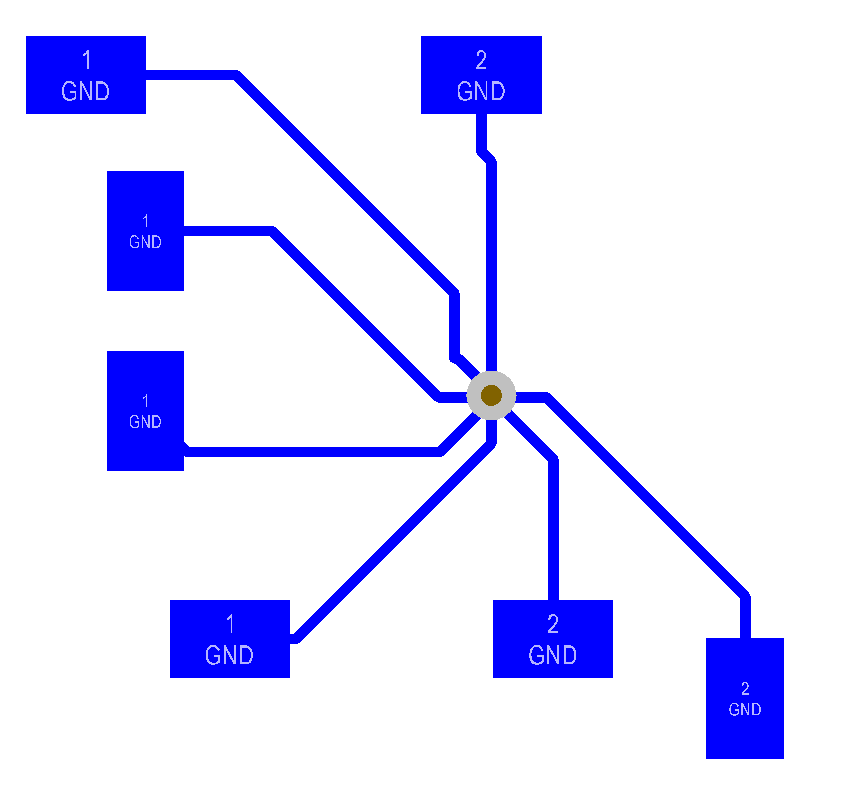
\includegraphics[width=0.8\textwidth]{fig/pcb/pcb_removing_vias.png}
  \caption{Removing vias}
  \label{fig:removingvias-pcb}
\end{figure}
 \TODO{Write about this figure}

Another reason has to do with the difference between our designs. Where the other group had to route only 1 memory chip, we had 5. This naturally made the routing much more complex.

Initially we attempted auto routing. This took just around 12 minutes before constraints were set. And the better part of half an hour, after the constraints were set. This showed us quite a few issues that needed to be handled, and even more so when we finally got the constraints in.

\TODO{Fill in about the types of errors/warnings we got.}
\begin{itemize}
\item Constraints violations set wrong.
\item Power-plane net-labeled wrong.
\item Clearance constraints violated by Altium.
\item Short-circuiting vias.
\item Overlapping vias.
\item In general, the auto-routing started to produce violations.
\item more\ldots
\end{itemize}
\TODO{Silk-over-silk in USB/Lenna, errors we could ignore.}
\TODO{Scaling of board. (Should go elsewhere or not at all?)}

Initially we started with a board size chosen more or less at random, and picked something that seemed to fit the components comfortably with room to spare.

After laying out the components on the board, we noticed that the board had quite a bit of room left over. As this would be a waste of resources, we scaled the board down in size. We did this by moving the keep-out-borders inwards until the wasted space was removed, and then used the ``scale-to-fit-components''-tool in Altium, with the Keepout-border selected.

In the end we remapped some pins to increase physical proximity, and to untangle the amount of crossing wires. Although care was taken during this process, we accidentally happened to disconnect one pin in the schematic while reordering. We did notice this before production, and were able to correct the mistake by manually routing the connection. Finally, we did some manual routing to reduce the amount of unnecessary vias.


We spent the entire final week before production working on the routing. In comparison, the energy group used only 2 days. There are quite a few possible reasons why we ended up using so much more time than them for this:

One of the reasons were simply that we were the first group to start routing. We thus got to fall into some gotcha-traps, with no one to warn us about them.

An example of such a trap was that we didn't set the correct Design Rules before auto-routing, until a few days into the week. This naturally didn't give us the routing that we wanted, and gave us a few headaches.

Related to this is the fact that we didn't experiment enough with different routing strategies. We wanted to reduce the number of vias, but went with the default routing in Altium. We then did quite an amount of manual routing to reduce the number of vias. Figure \ref{fig:removingvias-pcb} shows an example where we coupled together several pins to the same via going to the GND-layer. The amount of manual work could perhaps have been reduced by selecting the "Via Mixer" strategy instead.

\begin{figure}[h]
  \centering
  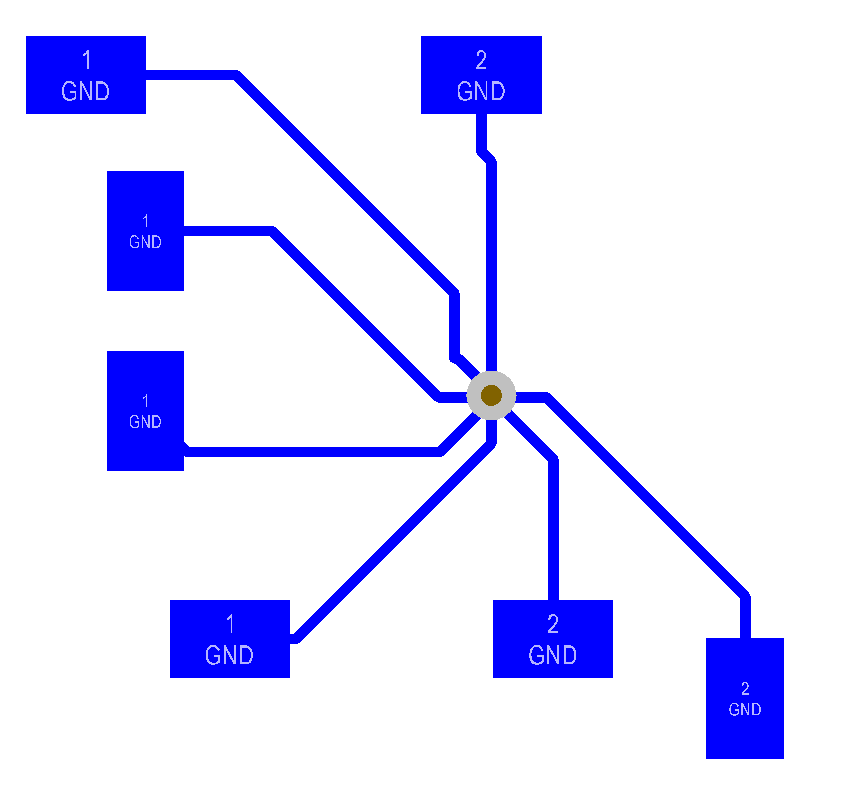
\includegraphics[width=0.8\textwidth]{fig/pcb/pcb_removing_vias.png}
  \caption{Removing vias}
  \label{fig:removingvias-pcb}
\end{figure}
 \TODO{Write about this figure}

Another reason has to do with the difference between our designs. Where the other group had to route only 1 memory chip, we had 5. This naturally made the routing much more complex.

Initially we attempted auto routing. This took just around 12 minutes before constraints were set. And the better part of half an hour, after the constraints were set. This showed us quite a few issues that needed to be handled, and even more so when we finally got the constraints in.

\TODO{Fill in about the types of errors/warnings we got.}
\begin{itemize}
\item Constraints violations set wrong.
\item Power-plane net-labeled wrong.
\item Clearance constraints violated by Altium.
\item Short-circuiting vias.
\item Overlapping vias.
\item In general, the auto-routing started to produce violations.
\item more\ldots
\end{itemize}
\TODO{Silk-over-silk in USB/Lenna, errors we could ignore.}
\TODO{Scaling of board. (Should go elsewhere or not at all?)}

Initially we started with a board size chosen more or less at random, and picked something that seemed to fit the components comfortably with room to spare.

After laying out the components on the board, we noticed that the board had quite a bit of room left over. As this would be a waste of resources, we scaled the board down in size. We did this by moving the keep-out-borders inwards until the wasted space was removed, and then used the ``scale-to-fit-components''-tool in Altium, with the Keepout-border selected.

In the end we remapped some pins to increase physical proximity, and to untangle the amount of crossing wires. Although care was taken during this process, we accidentally happened to disconnect one pin in the schematic while reordering. We did notice this before production, and were able to correct the mistake by manually routing the connection. Finally, we did some manual routing to reduce the amount of unnecessary vias.


We spent the entire final week before production working on the routing. In comparison, the energy group used only 2 days. There are quite a few possible reasons why we ended up using so much more time than them for this:

One of the reasons were simply that we were the first group to start routing. We thus got to fall into some gotcha-traps, with no one to warn us about them.

An example of such a trap was that we didn't set the correct Design Rules before auto-routing, until a few days into the week. This naturally didn't give us the routing that we wanted, and gave us a few headaches.

Related to this is the fact that we didn't experiment enough with different routing strategies. We wanted to reduce the number of vias, but went with the default routing in Altium. We then did quite an amount of manual routing to reduce the number of vias. The amount of manual work could perhaps have been reduced by selecting the "Via Mixer" strategy instead.

\TODO{Insert "via-hub" figure here}

Another reason has to do with the difference between our designs. Where the other group had to route only 1 memory chip, we had 5. This naturally made the routing much more complex.

Initially we attempted auto routing. This took just around 12 minutes before constraints were set. And the better part of half an hour, after the constraints were set. This showed us quite a few issues that needed to be handled, and even more so when we finally got the constraints in.

\TODO{Fill in about the types of errors/warnings we got.}
\begin{itemize}
\item Constraints violations set wrong.
\item Power-plane net-labeled wrong.
\item Clearance constraints violated by Altium.
\item Short-circuiting vias.
\item Overlapping vias.
\item In general, the auto-routing started to produce violations.
\item more\ldots
\end{itemize}
\TODO{Silk-over-silk in USB/Lenna, errors we could ignore.}
\TODO{Scaling of board. (Should go elsewhere or not at all?)}

Initially we started with a board size chosen more or less at random, and picked something that seemed to fit the components comfortably with room to spare.

After laying out the components on the board, we noticed that the board had quite a bit of room left over. As this would be a waste of resources, we scaled the board down in size. We did this by moving the keep-out-borders inwards until the wasted space was removed, and then used the ``scale-to-fit-components''-tool in Altium, with the Keepout-border selected.

In the end we remapped some pins to increase physical proximity, and to untangle the amount of crossing wires. Although care was taken during this process, we accidentally happened to disconnect one pin in the schematic while reordering. We did notice this before production, and were able to correct the mistake by manually routing the connection. Finally, we did some manual routing to reduce the amount of unnecessary vias.

